\documentclass{article}
\usepackage{graphicx} % Required for inserting images
\usepackage{amsmath,amssymb}
\usepackage{enumerate}
\usepackage{dcolumn}
\usepackage{bm}
\usepackage{microtype}
\usepackage{xcolor}


\definecolor{navyblue}{rgb}{0.0, 0.0, 0.5}
\usepackage{hyperref}
\usepackage{cleveref} 
\hypersetup{
    colorlinks=true,
    linktoc=all,
    allcolors=navyblue
}

\title{Axiverse Machine}
\author{Masha Baryakhtar, David Cyncynates, Ella Henry}
\date{\today}

\begin{document}

\maketitle
\section{Anthropics}
\subsection{$n$ heavy axions with uniform ICs}
The bounds for the possible ratio of the dark matter abundance to baryon abundance, $\zeta$, are given in \cite{ben} to be $2.5<\zeta <100$. The lower bound is related to the value for which perturbations near the size of our galaxy's stop growing, and the upper bound is related to the value that ultimately prevents star formation. All values within this range are allowed in the sense that they would lead to our existence today, but their likelihoods depend on the theory for dark matter, as we will see below. In section 5 of \cite{bookkeeping}, the authors consider the case of $n$ axions and the fraction of the dark matter that they constitute. If the axions make up all of the dark matter, then we can write $\zeta$ as:

\begin{equation}
\label{eq:zeta}
    \zeta = \sum_{a=1}^n c(m_a) F(\theta_a)
\end{equation}

Here, $c(m_a)F(\theta_a)$ is the fractional abundance in the $a$-th axion, where $F(\theta_a)$ encodes the dependence of the fractional abundance on the axion's intial misalignment angle. For small enough angles, $F(\theta_a)\sim\theta_a^2$. The $c(m_a)$ factor takes into account the fractional abundance's dependence on the mass and on the scale of symmetry breaking (e.g. for axions that start to oscillate during radiation domination, $c(m_a) \sim \Big(\frac{m_a}{H_{eq}}\Big)^{1/2}\Big(\frac{f_a}{M_{pl}}\Big)^2$).

The authors of \cite{bookkeeping} then calculate the probability of finding ourselves in a causal patch where the dark matter abundance is no larger than the observed value of $\zeta \sim 5$, without being so small that we could not exist, i.e. the probability that $2.5<\zeta<5$. They consider $n$ axions at the GUT scale ($f\sim 10^{16}$ GeV), with masses $m_a\geq10^{-21}$ eV, and find that this probability is:

\begin{equation}
\label{eq:prob-result}
    P_n = \frac{\int_{2.5}^5 \frac{d\zeta \zeta^{(n-2)/2}}{1+\zeta}}{\int_{2.5}^{100}\frac{d\zeta \zeta^{(n-2)/2}}{1+\zeta}} = \text{0.3, 0.16, 0.06, 0.02, 0.006, . . .}
\end{equation}

This result is independent of the masses $m_a$, as long as $m_a$ is large enough so that the axion is required to have small enough $\theta_a$ to not overproduce the dark matter. For such small angles, we can approximate the $\theta_a$ dependence of the relic abundance as $F(\theta_a)\sim \theta_a^2$. The exact mass threshold for which the result becomes independent of the mass depends on the decay constant; for $f_a \sim 10^{16}$ GeV, this corresponds to a mass of $m_a \sim  10^{-19}$ eV.

\subsection{2 axions of arbitrary mass and uniform ICs}
Focusing on two axions, we can take into account the mass dependence of the probability given in Eq. \eqref{eq:prob-result}, we have:

\begin{equation}
\label{eq:two-axion}
P_2 = \frac{\int_{2.5<\zeta<5} \frac{d\theta_1d\theta_2}{1+\zeta}}{\int_{2.5<\zeta<100} \frac{d\theta_1d\theta_2}{1+\zeta}}
\end{equation}

\noindent where $\zeta = c_1\theta_1^2+c_2\theta_2^2$ and $c_i = (m_i/H_{eq})^{1/2}(f/M_{pl})^2$.

\begin{figure}[h]
    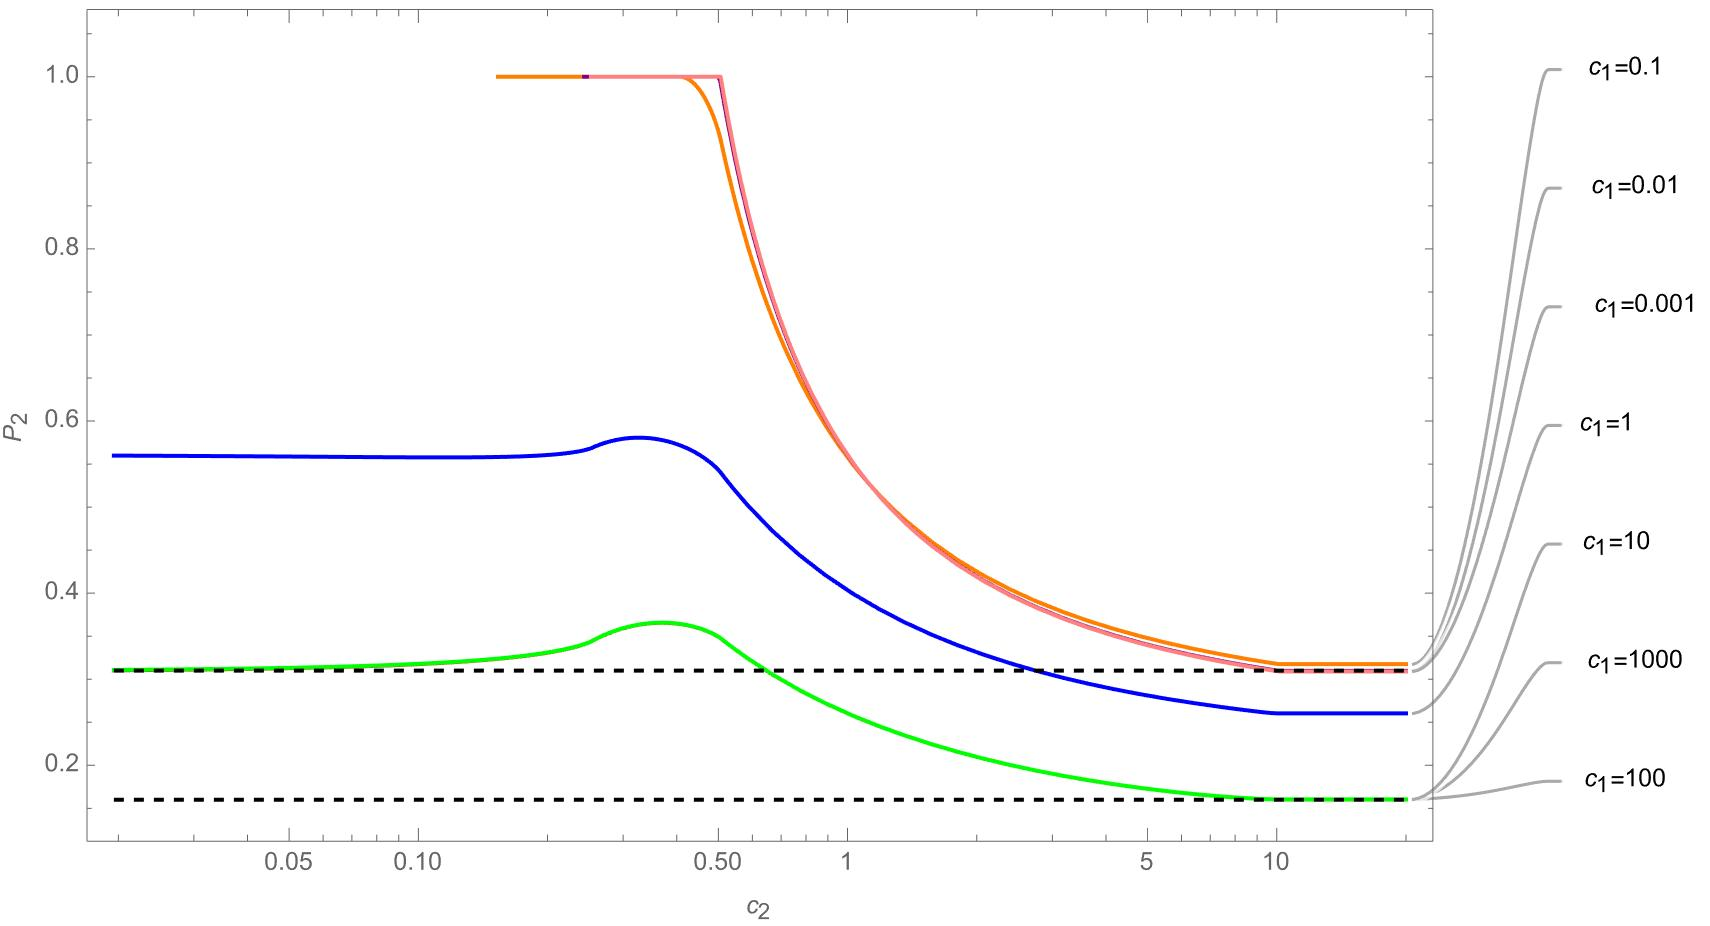
\includegraphics[scale=0.5]{figs/twoAxions.jpeg}
    \centering
    \caption{Probability of measuring $2.5<\zeta<5$ in the case of two axion as a function of $c_2$, for different values of $c_1$ (Eq. \eqref{eq:two-axion}). The dashed horizontal lines correspond to the probabilities for 1 and 2 axions as given by Eq. \eqref{eq:prob-result}: 0.3 and 0.16 respectively.}
\end{figure}

In the graph above, there seems to be some noticeable behavior around a value of $c\sim 10$, which I'll call $c_\text{crit}$. In the regimes where at least one $c_i > c_\text{crit}$ while the other is much smaller, or when both $c_\text{crit}$, correspond to the mass-independent regime to which Eq. $\eqref{eq:two-axion}$ is valid. If $\zeta_\text{lower}<\zeta<\zeta_\text{upper}$, then the value of $c_\text{crit} = \zeta_\text{upper}/\pi^2$ or $100/\pi^2\approx10$ in our case. In terms of the mass and decay constant of the $a$-th axion, this condition is (up to some order 1 numbers I think):

\begin{equation}
    \boxed{\left(\frac{m_a}{H_{eq}}\right)^{1/2}\left(\frac{f}{M_{pl}}\right)^{2}=\frac{\zeta_\text{upper}}{\pi^2}}
\end{equation}

This dependence of $c_\text{crit}$ on $\zeta_\text{upper}$ physically corresponds to the idea that the upper anthropic limit on the dark matter abundance affects the value of $c$ that an axion must have in order to contribute meaningfully to that abundance. Note that if the misalignment angle is large enough so that the dependence of the energy density on it is different from quadratic, then this expression for $c_\text{crit}$ will be slightly modified. \\

\noindent \textbf{Things to better understand:}
\begin{enumerate}
    \item include correction to the energy density from cosine potential if you want to integrate over all angles equally and get rid of requirement imposed by looking at only heavy masses
    \item what happens below $c_\text{crit}$
    \item and related to the previous point, what the bump is, what it looks like with more axions
\end{enumerate}

\subsection{1 axion with arbitrary scale of inflation}

\begin{figure}[h]
\label{fig:1axion-unifprob}
    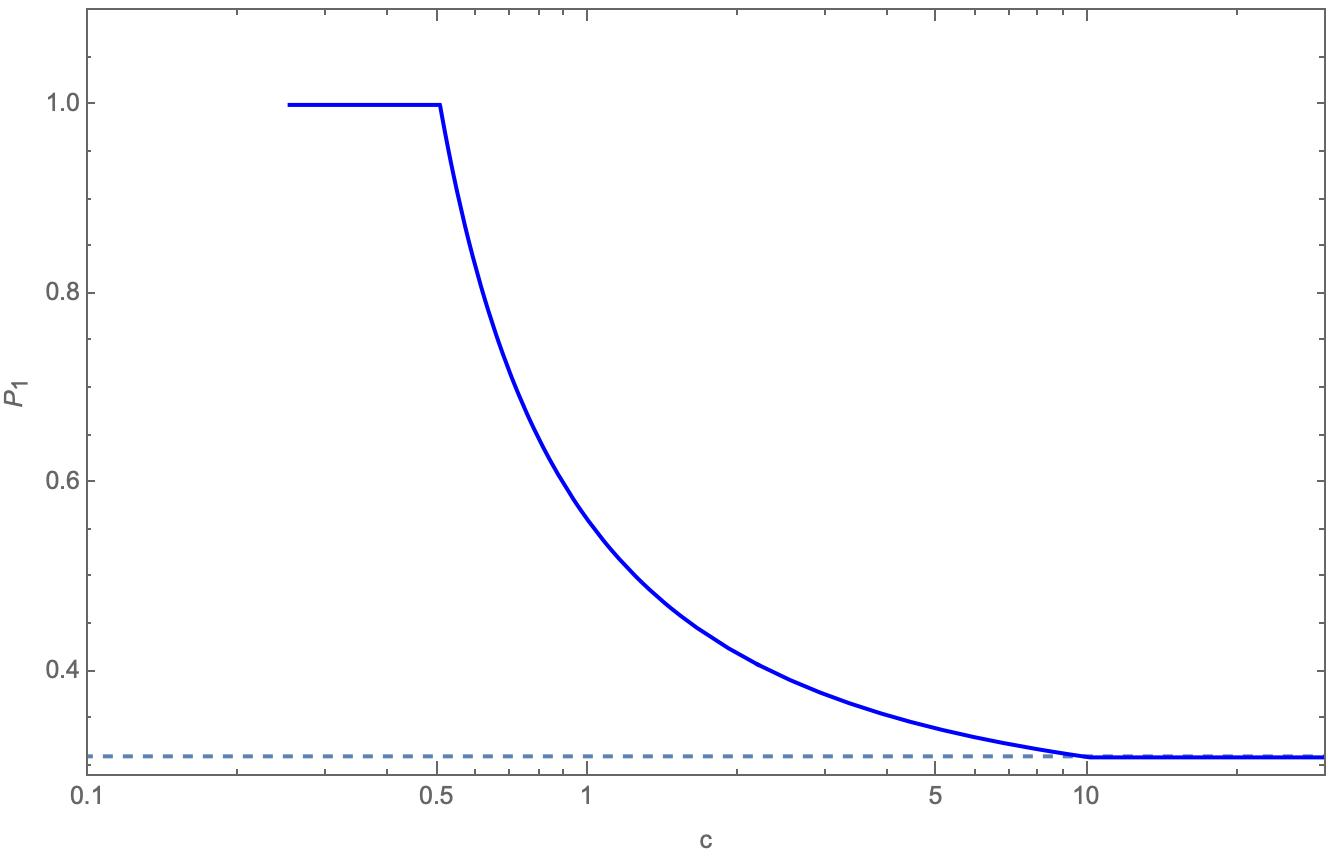
\includegraphics[scale=0.5]{figs/oneAxion.jpeg}
    \centering
    \caption{Probability of measuring $2.5<\zeta<5$ in the case of one axion as a function of $c$. The dashed line corresponds to the mass-independent probability from Eq. \eqref{eq:prob-result} for $n=1$.}
\end{figure}

First, consider a single axion in a scenario with a high scale of inflation such that its misalignment angle is uniformly distributed between $[-\pi,\pi]$. In the anthropic measure, we can again calculate the probability that $2.5<\zeta=c\theta^2<5$ for this single axion and plot this probability as a function of $c$, as shown above:

\begin{equation}
\label{eq:1axion-prob}
   P_1 = \frac{\int_{2.5<\zeta<5} \frac{d\theta}{1+\zeta}}{\int_{2.5<\zeta<100} \frac{d\theta}{1+\zeta}} = \frac{\int_{-\pi}^{\pi}\frac{d\theta}{1+c\theta^2}H(c\theta^2-2.5)H(5-c\theta^2)}{\int_{-\pi}^{\pi}\frac{d\theta}{1+c\theta^2}H(c\theta^2-2.5)H(100-c\theta^2)}
\end{equation}

\noindent where $H(\theta)$ is the Heaviside step function. The 1-axion probability as shown in the above figure follows the same story as the one we deduced from the 2-axion scenario, in which an axion contributed once its value of $c$ satisfies $c>c_\text{crit}$.

For an arbitrary scale of inflation, if the duration of inflation is long enough, the initial conditions are drawn according to the following distribution:

\begin{equation}
\label{eq:inflationary-dist}
    p(\theta) \propto \exp{\left(-\frac{8\pi^2V(\theta)}{3H^4}\right)}
\end{equation}

\noindent where $V(\theta)$ is the potential. To study the effect of inflationary initial conditions on anthropics, we can take two approaches: (1) an exact calculation of the probability, with the integrand integrated against the exponential distribution for $\theta$ from inflation; and (2) approximate the potential $V(\theta)$ as a quadratic so that the distribution in Eq. \eqref{eq:inflationary-dist} is a Gaussian with some standard deviation $\sigma$, and the approximate the Gaussian as flat between $[-\sigma,\sigma]$.

\subsubsection{Exact approach}

\begin{figure}[h]
    \centering
    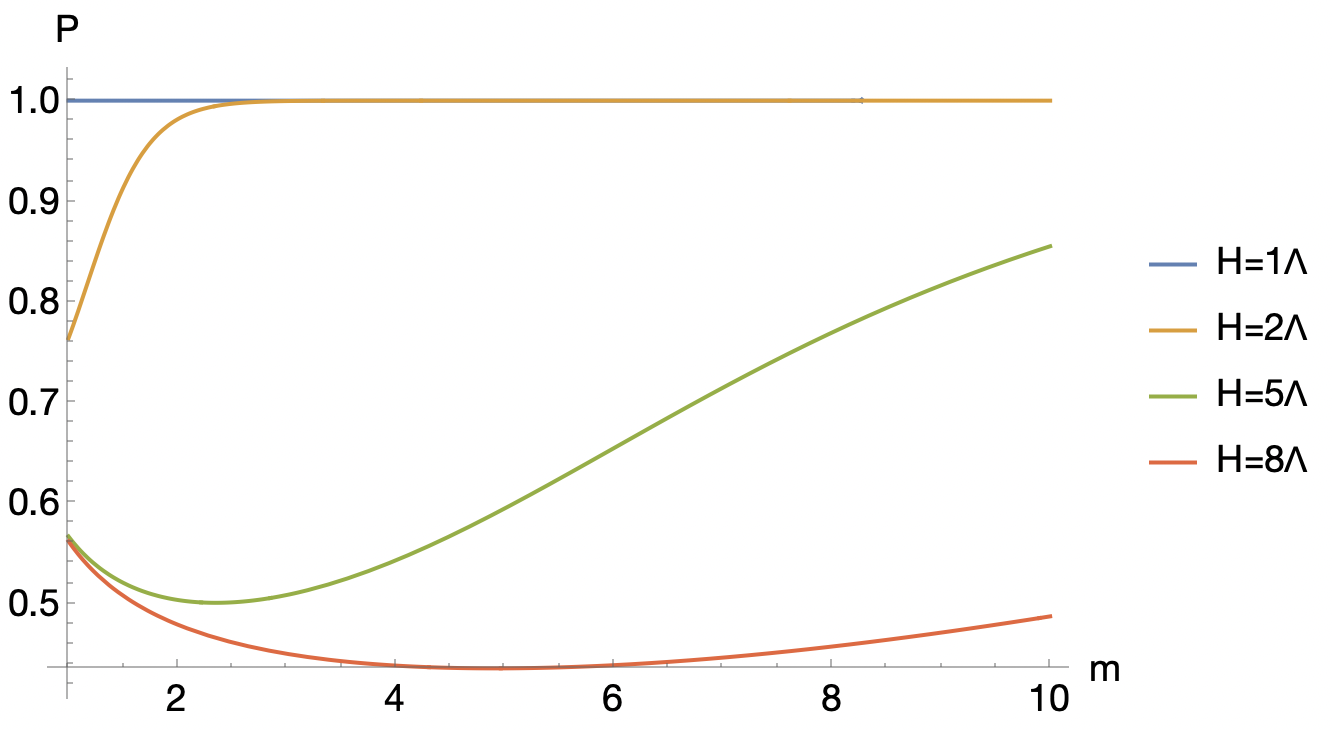
\includegraphics[width=1
\linewidth]{figs/Screenshot 2025-07-14 at 17.00.25.png}
    \caption{Probability of $2.5<\zeta<5$ for a stochastic axion scenario, with different vales of $H$ relative to $\Lambda = (mf)^{1/2}$}
    \label{fig:enter-label}
\end{figure}

Solving exactly\footnote{``exactly" in the sense that I'm not approximating the potential or distribution of misalignment angles, but integral is done numerically.} for the anthropic probability with initial conditions can be done pretty straightforwardly for one axion. The probability becomes:

\begin{equation}
    \label{eq:inflation-prob-1axion}
    P = N^{-1}\int_{2.5<\zeta<5} \frac{d\theta}{1+\zeta} \exp{\left(-\frac{8\pi^2V(\theta)}{3H^4}\right)}
\end{equation}

\noindent where the normalization is $N = \int_{2.5<\zeta<100} \frac{d\theta}{1+\zeta}\exp{\left(-\frac{8\pi^2V(\theta)}{3H^4}\right)}$. This probability is plotted against $\sqrt{mf}$ for certain values of $H$ in the figure above. As expected, for each curve, we see that when the scale of inflation is low relative to the size of the potential (i.e. $H<\Lambda$), the probability that $2.5<\zeta<5$ grows, since you are sampling $\theta$ from a distribution peaked closer and closer to zero (effectively acts like a small $c$, see Fig. 3). When $H>\Lambda$, you recover the expected behavior from flat initial conditions: the probability drops for $\Lambda$ (until $\Lambda \sim H$, and then you enter the first regime).


\subsubsection{Approximate approach}
Alternatively, we can study the effect of inflationary initial conditions on the anthropic probability by approximating the distribution in Eq. \eqref{eq:inflation-prob-1axion} as $\theta \sim \text{Unif}(-\sigma,\sigma)$ where $\sigma = \sqrt{(3H^4)/(8\pi^2m^2f^2})$. Then, the expression for the probability is the same as in Eq. \eqref{eq:1axion-prob}, except the bounds of integration over $\theta$ are different. We can perform a change of variables $\theta\rightarrow\frac{\sigma}{\pi}\theta'$ so that this difference manifests itself not in the bounds of integration but in the $c$ factor:

\begin{align*}
    \label{eq:approx-inf-prob}
    P & = \frac{\int_{-\sigma}^{\sigma}\frac{d\theta}{1+c\theta^2}H(c\theta^2-2.5)H(5-c\theta^2)}{N'} \\
    & = \frac{\int_{-\pi}^{\pi}\frac{d\theta'}{1+c(\frac{\sigma}{\pi}\theta')^2}H(c(\frac{\sigma}{\pi}\theta')^2-2.5)H(5-c(\frac{\sigma}{\pi}\theta')^2)}{N'}
\end{align*}

\noindent As usual, the normalization factor $N'$ is the same integral but with an upper limit $c\theta^2<100$. The integral in the last line is the same as that in Eq. \eqref{eq:1axion-prob}, but with $c\rightarrow c(\sigma/\pi)^2 = \frac{c}{\pi^2}(3H^4)/(8\pi^2m^2f^2)$. 

The nice thing about this approach is that it generalizes nicely to $n>1$ axions, whereas the exact approach in the previous section would be harder to think about for $n>1$.

So to summarize, if we approximate the potential to be quadratic (i.e. $H_I<\Lambda$), and then approximate the distribution of initial conditions to be flat between $\pm \sqrt{(3H^4)/(8\pi^2m^2f^2})$, then the condition for an axion to contribute to the anthropic measure is:

\begin{equation}
    \boxed{\frac{3}{8\pi^2}\frac{H_I^4}{M_{pl}^2H_{eq}^{1/2}m^{3/2}}=\zeta_\text{upper}}
\end{equation}

\section{GSification}

\appendix
\section{Introduction}
Consider the general task of determining how the initial condition of a collection of scalar fields $\bm \theta(0)$ maps onto the final partition of energy density among the various mass eigenstates, where the dynamics are controlled by the following Lagrangian:
\begin{align}\label{eqn:fundamental}
    {\cal L} = \frac{1}{2}\dot{\bm \theta}^T {\bm K}\dot{\bm\theta} - V(\bm\theta)\,.
\end{align}
The kinetic term matrix $\bm K$ may be diagonalized through the following field redefinition
\begin{align}
    \bm\psi \equiv \bm F \bm R^T \bm\theta\,,\hspace{1cm}\bm F^2\equiv \bm R^T \bm K \bm R\,,
\end{align}
where $\bm R^T \bm R  = 1$, and $\bm F^2$ is the diagonal matrix of $\bm K$ eigenvalues. In this basis, the Lagrangian becomes
\begin{align}\label{eqn:canonical}
    {\cal L} = \frac12\dot{\bm\psi}^T\dot{\bm\psi} - V(\bm R\bm F^{-1}\bm\psi)\,.
\end{align}
Although one may as well have started with \Cref{eqn:canonical}, starting with \Cref{eqn:fundamental} is essential if the form of $V$ is specified, since mixing induced by the off-diagonal kinetic terms will play an important role in the dynamics.

The potential $V(\bm\psi)\equiv V(\bm R\bm F^{-1}\bm\psi)$ is in general an arbitrarily complicated function of the fields, and it may have multiple, physically inequivalent minima, from which $\bm\psi$ may be initialized arbitrarily far away. Therefore, at early times there is no sense in which one may define any particular linear combination of the fields to carry some definite fraction of the energy density of the system. Only at asymptotically late times is one guaranteed that the fields settle into a local minimum of the potential, though I emphasize that one does not know the location or curvature of this part of the potential \emph{a priori}. Therefore, our algorithm to separate out the various late-time mass eigenstates of the fields must avoid making explicit reference to the shape of the potential about any particular point.


\subsection{Separable energy density}\label{sec:separable-energy-density}
To simplify notation, we will use $\bm V''$ and $\bm V'$ to refer to the second and first derivatives $\partial^2 V(\bm\psi)/\partial\bm\psi\partial\bm\psi$ and $\partial V(\bm\psi)/\partial\bm\psi$ respectively. The matrix $\bm V''$ defines the square of the local mass eigenvalues, and so we must redefine the fields to work in the mass eigenstates:
\begin{align}
    \bm\phi\equiv \bm S^T\bm\psi \,,\hspace{1cm} \bm M^2\equiv \bm S^T\bm V''(\psi)\bm S\,,
\end{align}
where $\bm S^T\bm S = 1$ and $\bm M^2$ is the diagonal matrix of $\bm V''(\psi)$ eigenvalues. The energy density contained in the field oscillations is then
\begin{align}
    \rho_{\rm tot}\equiv \frac12 \dot{\bm\phi}^T\dot{\bm\phi} + \frac12 (\bm\phi - \bm\phi_0)\bm M^2(\bm\phi - \bm\phi_0)\,,
\end{align}
where $\bm\phi_0$ is the location of the minimum of the potential, which approximately satisfies
\begin{align}
    0&=\bm V''(\bm\psi)(\bm \psi - \bm\psi_0) + \bm V'(\psi) = \bm S \bm M^2 (\bm\phi - \bm \phi_0) + \bm S\bm V'(\bm\phi)
\end{align}
Thus, the energy density is
\begin{align}
    \rho_{\rm tot}\equiv \frac12 \dot{\bm\phi}^T\dot{\bm\phi} + \frac12\bm V'(\bm\phi)^T\bm M^{-2}\bm V'(\bm\phi)\,.
\end{align}
Labeling each of the mass eigenstates by their mass eigenvalue $m$, we may decompose the energy density:
\begin{align}\label{eqn:separated-energy-densities}
    \rho_{m}\equiv \frac12 \dot{\bm\phi}_m^2 + \frac12 [\bm M^{-2}(\bm V'(\bm\phi))^2]_m\,.
\end{align}
I assume a convention where the modes are sorted from lightest to heaviest, with $m = m_0$ being the lightest eigenvalue and $m_{-1}$ the heaviest.

\subsection{Pruning trivial modes}
The procedure of \Cref{sec:separable-energy-density} is sufficient to determine the final partition of energy densities at asymptotically late times. In practice, integrating the equations of motion to very late times where one may assume that all states have settled to the bottom of some local minimum is impossible if the masses span more than a few orders of magnitude, since the number of time steps that must be taken is proportional to the ratio of the largest to smallest masses. On the other hand, heavy particles will settle to the minimum of their potential long before the lightest mass eigenstates have begun to oscillate, and so we may remove them from the integration by carefully checking that these modes are dynamically decoupled from all others.

To eliminate the heavy modes, it is enough to replace the damping term $3 H \dot{\bm \phi}_{m_i}$ with the critically damped term $2m_i\dot{\bm \phi}_{m_i}$. Note, though, that at every step, the heavy modes will still involve the heavy mass scale. Therefore, one should re-scale the heavy-mode EOM by the mass (squared) of the lightest mode that has been integrated out. This will keep the heavy modes dynamically forced to the bottom of their potentials, while removing any fast timescales.

\section{Coupling to photons}
In the interaction basis, there is a single mode that couples to photons, which we take to be $\theta_1$ without loss of generality:
\begin{align}
    {\cal L}_{\rm int} = \frac{\alpha_{\rm EM}}{8\pi}\theta_1\tilde F F =\frac{\alpha_{\rm EM}}{8\pi} [\bm R\bm F^{-1}\bm S \bm \phi]_1 \tilde F F.
\end{align}
For each mass eigenstate, the coupling to the photon is then given by the corresponding coefficient in the first row of this matrix.

\begin{figure}
    \centering
    \includegraphics[width=1\linewidth]{figs/Screenshot 2024-11-12 at 5.53.04 PM.png}
    \caption{This is a simulation of the trivial case where each axion has its own instanton and the kinetic term is diagonal. The blue line represents the expectation that $\rho\propto m^{1/2}$. The horizontal axis is the log of the masses normalized against some arbitrary mass scale, while the vertical axis is the asymptotic relic abundance of each mass eigenstate normalized against some arbitrary energy density.}
    \label{fig:enter-label}
\end{figure}
\begin{figure}
    \centering
    \includegraphics[width=1\linewidth]{figs/Screenshot 2024-11-12 at 5.53.09 PM.png}
    \caption{40 axions!}
    \label{fig:enter-label}
\end{figure}
\begin{figure}
    \centering
    \includegraphics[width=1\linewidth]{figs/Screenshot 2024-11-12 at 5.53.14 PM.png}
    \caption{20 axions!}
    \label{fig:enter-label}
\end{figure}

\section{Directions}
\begin{enumerate}
    \item Plot: $g_{a\gamma\gamma}\sqrt{\rho/\rho_{\rm DM}}$ vs mass (like what we have in the friendship paper) for all the axions.
    \item Theoretical expectation for thermalization rate of nonlinearly coupled chain of oscillators -- extend to time-varying parameters with adiabatic approximation
    \item Theoretical expectations for the distribution of energy density among the mass eigenstates
    \item Effect of QCD Axion?
    \item Statistics of the CC (what is the distribution of vacuum energies?)
\end{enumerate}

\section{Being more clever}
Let us consider the algorithm more carefully, and consider how it may be improved.
\begin{enumerate}
    \item Heavy modes are still kept. Can we drop them entirely using an analytical method without introducing numerical error? Perhaps we simply don't include them in the rotation matrix?
    \item Light modes are included in the rotation matrix even though they don't need to be included. Perhaps only including the oscillating modes in the rotation matrix would improve numerical stability.
    \item In order to avoid using arbitrary precision during numerical integration, consider why arbitrary precision may be considered necessary at all. It is only the case that arbitrary precision would be necessary if terms with a huge dynamical range entered into the light field equations of motion in the first place. These terms necessarily cancel -- how can we eliminate them without losing precision? IDEA: Suppose there are N dynamical degrees of freedom -- using arbitrary precision, precompute an N dimensional subvolume of the potential
\end{enumerate}


\end{document}